%!TeX encoding = UTF-8
%!TeX program = xelatex
\documentclass[notheorems, aspectratio=54]{beamer}
% aspectratio: 1610, 149, 54, 43(default), 32
\usepackage{hyperref}

 
\usepackage{latexsym}
\usepackage{amsmath,amssymb}
\usepackage{mathtools}
\usepackage{color,xcolor}
\usepackage{graphicx}
\usepackage{algorithm}
\usepackage{amsthm}
\DeclareMathOperator*{\argmax}{argmax} % thin space, limits underneath in displays
\usepackage{lmodern} % 解决 font warning
% \usepackage[UTF8]{ctex}
\usepackage{animate} % insert gif

\usepackage{lipsum} % To generate test text 
\usepackage{ulem} % 下划线,波浪线

\usepackage{listings} % display code on slides; don't forget [fragile] option after \begin{frame}

% ----------------------------------------------
% tikx
\usepackage{framed}
\usepackage{fancybox}
\usepackage{tikz}
\usepackage{pgf}
\usetikzlibrary{automata, calc,trees,positioning,arrows,chains,shapes.geometric,%
    decorations.pathreplacing,decorations.pathmorphing,shapes,%
    matrix,shapes.symbols}
\pgfmathsetseed{1} % To have predictable results
% Define a background layer, in which the parchment shape is drawn
\pgfdeclarelayer{background}
\pgfsetlayers{background,main}

% define styles for the normal border and the torn border
\tikzset{
  normal border/.style={orange!30!black!10, decorate, 
     decoration={random steps, segment length=2.5cm, amplitude=.7mm}},
  torn border/.style={orange!30!black!5, decorate, 
     decoration={random steps, segment length=.5cm, amplitude=1.7mm}}}

% Macro to draw the shape behind the text, when it fits completly in the
% page
\def\parchmentframe#1{
\tikz{
  \node[inner sep=2em] (A) {#1};  % Draw the text of the node
  \begin{pgfonlayer}{background}  % Draw the shape behind
  \fill[normal border] 
        (A.south east) -- (A.south west) -- 
        (A.north west) -- (A.north east) -- cycle;
  \end{pgfonlayer}}}

% Macro to draw the shape, when the text will continue in next page
\def\parchmentframetop#1{
\tikz{
  \node[inner sep=2em] (A) {#1};    % Draw the text of the node
  \begin{pgfonlayer}{background}    
  \fill[normal border]              % Draw the ``complete shape'' behind
        (A.south east) -- (A.south west) -- 
        (A.north west) -- (A.north east) -- cycle;
  \fill[torn border]                % Add the torn lower border
        ($(A.south east)-(0,.2)$) -- ($(A.south west)-(0,.2)$) -- 
        ($(A.south west)+(0,.2)$) -- ($(A.south east)+(0,.2)$) -- cycle;
  \end{pgfonlayer}}}

% Macro to draw the shape, when the text continues from previous page
\def\parchmentframebottom#1{
\tikz{
  \node[inner sep=2em] (A) {#1};   % Draw the text of the node
  \begin{pgfonlayer}{background}   
  \fill[normal border]             % Draw the ``complete shape'' behind
        (A.south east) -- (A.south west) -- 
        (A.north west) -- (A.north east) -- cycle;
  \fill[torn border]               % Add the torn upper border
        ($(A.north east)-(0,.2)$) -- ($(A.north west)-(0,.2)$) -- 
        ($(A.north west)+(0,.2)$) -- ($(A.north east)+(0,.2)$) -- cycle;
  \end{pgfonlayer}}}

% Macro to draw the shape, when both the text continues from previous page
% and it will continue in next page
\def\parchmentframemiddle#1{
\tikz{
  \node[inner sep=2em] (A) {#1};   % Draw the text of the node
  \begin{pgfonlayer}{background}   
  \fill[normal border]             % Draw the ``complete shape'' behind
        (A.south east) -- (A.south west) -- 
        (A.north west) -- (A.north east) -- cycle;
  \fill[torn border]               % Add the torn lower border
        ($(A.south east)-(0,.2)$) -- ($(A.south west)-(0,.2)$) -- 
        ($(A.south west)+(0,.2)$) -- ($(A.south east)+(0,.2)$) -- cycle;
  \fill[torn border]               % Add the torn upper border
        ($(A.north east)-(0,.2)$) -- ($(A.north west)-(0,.2)$) -- 
        ($(A.north west)+(0,.2)$) -- ($(A.north east)+(0,.2)$) -- cycle;
  \end{pgfonlayer}}}

% Define the environment which puts the frame
% In this case, the environment also accepts an argument with an optional
% title (which defaults to ``Example'', which is typeset in a box overlaid
% on the top border
\newenvironment{parchment}[1][Example]{%
  \def\FrameCommand{\parchmentframe}%
  \def\FirstFrameCommand{\parchmentframetop}%
  \def\LastFrameCommand{\parchmentframebottom}%
  \def\MidFrameCommand{\parchmentframemiddle}%
  \vskip\baselineskip
  \MakeFramed {\FrameRestore}
  \noindent\tikz\node[inner sep=1ex, draw=black!20,fill=white, 
          anchor=west, overlay] at (0em, 2em) {\sffamily#1};\par}%
{\endMakeFramed}

% ----------------------------------------------

\mode<presentation>{
    \usetheme{CambridgeUS}
    % Boadilla CambridgeUS
    % default Antibes Berlin Copenhagen
    % Madrid Montpelier Ilmenau Malmoe
    % Berkeley Singapore Warsaw
    \usecolortheme{beaver}
    % beetle, beaver, orchid, whale, dolphin
    \useoutertheme{infolines}
    % infolines miniframes shadow sidebar smoothbars smoothtree split tree
    \useinnertheme{circles}
    % circles, rectanges, rounded, inmargin
}
% 设置 block 颜色
\setbeamercolor{block title}{bg=red!30,fg=white}

\newcommand{\reditem}[1]{\setbeamercolor{item}{fg=red}\item #1}

% 缩放公式大小
\newcommand*{\Scale}[2][4]{\scalebox{#1}{\ensuremath{#2}}}

% 解决 font warning
\renewcommand\textbullet{\ensuremath{\bullet}}

% ---------------------------------------------------------------------
% flow chart
\tikzset{
    >=stealth',
    punktchain/.style={
        rectangle, 
        rounded corners, 
        % fill=black!10,
        draw=white, very thick,
        text width=6em,
        minimum height=2em, 
        text centered, 
        on chain
    },
    largepunktchain/.style={
        rectangle,
        rounded corners,
        draw=white, very thick,
        text width=10em,
        minimum height=2em,
        on chain
    },
    line/.style={draw, thick, <-},
    element/.style={
        tape,
        top color=white,
        bottom color=blue!50!black!60!,
        minimum width=6em,
        draw=blue!40!black!90, very thick,
        text width=6em, 
        minimum height=2em, 
        text centered, 
        on chain
    },
    every join/.style={->, thick,shorten >=1pt},
    decoration={brace},
    tuborg/.style={decorate},
    tubnode/.style={midway, right=2pt},
    font={\fontsize{10pt}{12}\selectfont},
}
% ---------------------------------------------------------------------

% code setting
\lstset{
    language=C++,
    basicstyle=\ttfamily\footnotesize,
    keywordstyle=\color{red},
    breaklines=true,
    xleftmargin=2em,
    numbers=left,
    numberstyle=\color[RGB]{222,155,81},
    frame=leftline,
    tabsize=4,
    breakatwhitespace=false,
    showspaces=false,               
    showstringspaces=false,
    showtabs=false,
    morekeywords={Str, Num, List},
}

% ---------------------------------------------------------------------

%% preamble
\title{Lecture 08}
% \subtitle{The subtitle}
\author{Dihui Lai}
\institute[WUSTL]{dlai@wustl.edu}

% -------------------------------------------------------------

\begin{document}

%% title frame
\begin{frame}
    \titlepage
\end{frame}


\begin{frame}
\begin{center}
Multi-class Classification
\end{center}
\end{frame}

\begin{frame}
\frametitle{Multinomial Distribution }
Multinomial distribution: there could be $\mathnormal{c}$ outcome of an experiment, each of probability  $\mathnormal{p_1}$, $\mathnormal{p_2}$, $\mathnormal{p_3}$, ..., $\mathnormal{p_k}$ and $\mathnormal{\sum\limits_{k=1}^c p_k=1}$. If one perform $\mathnormal{M}$ experiments, the probability of getting $\mathnormal{m_1}$, $\mathnormal{m_2}$, $\mathnormal{m_3}$, ... $\mathnormal{m_c}$ of each out come can be described as 
$$\mathnormal{f(m_1, m_2, m_3, ... m_c)=\frac{M!}{m_1! m_2! ... m_c!} p_1^{m_1} p_2^{m_2} ... p_c^{m_c}}$$
\end{frame}


\begin{frame}
\frametitle{Multi-class Classification}
If a target variable contains more than 2 types of out come, logistic regression can not handle it easily. We need to build a \textbf{multi-class classification} model 

Assume there can be C possible outcome in your target variable, we can use one-hot encoding and denote the out come of $\mathnormal{i^th}$ data point $\mathnormal{\vec{y}^i=[y_1^i, y_2^i, ... y_C^i]}$, only one element out of C is 1.
\end{frame}

\begin{frame}

\frametitle{Multi-class Classification: Likelihood Function}
For each data point $\mathnormal{i}$, the likelihood function can be constructed as 
$\mathnormal{L^i=\prod \limits_{k=1}^C {p^{i}_{k}}^{y^i_k}}$ i.e. multinomial distribution of (M=1). For an outcome of class c, we have $\mathnormal{y_c}=1$ and all other elements of $\mathnormal{y}$ are 0. $\mathnormal{y_1=0}$, $\mathnormal{y_2=0}$, ....$\mathnormal{y_C=0}$. The log-likelihood of the dat point is $\mathnormal{ \ell^i=\sum\limits_{k=1}^C y^i_k \log(p^i_k)}$

The log-likelihood function (a.k.a log-loss) is
$$\mathnormal{\ell=\log(L)=\sum\limits_{i=1}^n \sum\limits_{k=1}^C y_k^i \log(p^i_k)}$$
\end{frame}

\begin{frame}
\frametitle{Multi-Class classification: Softmax }
To estimate $\mathnormal{p^i_k}$, we use softmax function of $\mathnormal{\vec{x} \cdot \vec{\beta}_k}$
$$\mathnormal{p^i_k=\frac{e^{\vec{x}^i \cdot \vec{\beta}_k}}{\sum\limits_{k=1}^C e^{\vec{x}^i \cdot \vec{\beta}_k}}}$$
\end{frame}

\begin{frame}
\frametitle{Multi-Class classification: Optimization }
To find the $\vec{\beta}_k$, we need to solve 

$$\frac{\partial{\ell}}{\partial \beta_{kj}}=0$$

Python method: \textit{"statsmodels.api.MNLogit"}
\end{frame}



\section{Naive Bayes Classifier}

\begin{frame}
\begin{center}
Naive Bayes Classifier
\end{center}
\end{frame}

\begin{frame}
\frametitle{Bayes' Theorem}
\textbf{Bayes' Theorem}: given two random variables $X$ and $Y$, the conditional probability of $X$ given $Y$ is expressed as:
$$P(Y\mid X)=\frac {P(X\mid Y)P(Y)}{P(X)}$$

Useful terminologies to interpret the equations: $P(Y)$ is called prior, which is the belif in Y without any other knowledge. $P(Y\mid X)$ is the posterior taking into consideration of X. $P(X\mid Y)$ is the likelihood.\\
\vspace{0.5cm}
In a discrete case, the probability distribution of $X$ can be calculated as
$P(X)=\sum _{i}P(X\mid Y_{i})P(Y_{i})$

\end{frame}

\begin{frame}
\frametitle{Baye's Theorem Example}
\begin{parchment}[Rain in California]
You are planning a trip to california tomorrow. Unfortunately, the weatherman has predicted rain for tomorrow. You know in southern california, it only rains 5 days each year and there is a chance the weather man makes false predictions. You searched on line and find that when it rains, the weatherman correctly forecasts rain of 90\% of the time. When it doesn't rain, he incorrectly forecasts rain 10\% of the time. What is the probability that it will rain tomorrow. 
\end{parchment}
\end{frame}

\begin{frame}
\frametitle{Baye's Theorem Example}
\textbf{Solution}: Denote the event that the weatherman forcast a raining day as F. The probability of rain given weatherman's forcast is $$P(1 \mid F)=\frac{P(1)P(F\mid 1)}{P(F)}$$. 

Given that we have $P(F \mid 1)=0.9$, $P(F\mid 0)=0.1$, $P(1)=\frac{5}{365}$ and $P(0)=1-P(1)= \frac{360}{365}$. $P(F)=P(F|1)P(1)+P(F|0)P(0)$,
Therefore, 
$$P(1 \mid F)=\frac{P(1)P(F\mid 1)}{P(F)}=\frac{\frac{5}{365}\cdot0.9}{0.1109}=0.111$$
\end{frame}

\begin{frame}

\frametitle{Joint Probability Distribution and Chain Rule}

\begin{itemize}
\item The joint probability distrution of two events can be discribed as $$P(A, B)=P(A\mid B)P(B)=P(B \mid A)P(A)$$

If $A$ and $B$ are two indpendent events, then we have $P(B)=P(B\mid A)$ and $P(A)=P(A\mid B)$

\vspace{0.5cm}

\item \textbf{Chain Rule}: Considering n random events $X_1$, $X_2$, $X_3$ ... $X_n$, their joint probability distribution can be described as
\begin{align*}
&P(X_n, \ldots, X_1)\\
&=P(X_{n}|X_{n-1},\ldots ,X_{1})P(X_{n-1},\ldots ,X_{1})\\
&=P(X_{n}|X_{n-1},\ldots ,X_{1})P(X_{n-1}|X_{n-2},\ldots ,X_{1})P(X_{n-2},\ldots ,X_{1})\\
&=...
\end{align*}
\end{itemize}
\end{frame}



\begin{frame}
\frametitle{Naive Bayes Classifier}
The joint probability distribution of predictor $\vec{x}$ and target variable $y$ can be written as
\begin{align*}
&p(x_1, x_2, ...x_n, y)\\
&=p(x_1|x_2, x_3, ..., y)p(x_2, x_3, ..., y)\\
&=p(x_1|x_2, x_3, ..., y)p(x_2|x_3, x_4, ..., y)p(x_3, x_4, ..., y)\\
&=p(x_1|x_2, x_3, ..., y)p(x_2|x_3, x_4, ..., y)...p(x_{n-1}|x_n, y)p(x_n|y)p(y)
\end{align*}


Assuming features are indepedent of each other but only dpendent on the target variable, then we have
$$
p(x_1, x_2, ...x_n, y)=p(y)\prod\limits_{i=1}^{N}p(x_i|y)
$$
\end{frame}


\begin{frame}
    \frametitle{Naive Bayes Classifier}
Using Bayes' theorem, we can get the conditional probability distribution of the target variable as
$$
p(Y|X)=\frac{p(X,Y)}{p(X)}
$$
Therefore, we have 
$$
p(Y|X)=\frac{p(y)\prod\limits_{i=1}^{N}p(x_i|y)}{\sum\limits_{y}p(y)\prod\limits_{i=1}^{N}p(x_i|y)}
$$

The denominator is constant if the features are know. $p(y)$ and $p(x_i\mid y)$ can be calculated from the data. We need to find the y that maximize the $p(Y\mid X)$, i.e.

$$
\hat{y}=\argmax_{y}p(y)\prod\limits_{i=1}^{N}p(x_i|y)
$$

\end{frame}


\begin{frame}
\begin{center}
Nature Language Process
\end{center}
\end{frame}

\section{Word Semantics and Vector Representations}
\begin{frame}
\frametitle{Word Semantics and Representations}
\begin{itemize} 
\item Homonymous: a word can have multiple definitions e.g. mouse could mean small rodents or it could mean computer devices. 
\item Synonyms/antonym (words' relations): couch/sofa, vomit/throw up, filbert/hazelnut; long/short, big/little
\item Word sentiments
\item Can we represent a word using vectors and quantify those measures?
\end{itemize}

\end{frame}



\begin{frame}

\frametitle{Word Vector Representations}
Term-term matrix or word-word matrix: count the number of times a word occurs in a context window around the target word (e.g. $\pm 7$)

sugar, a sliced lemon, a tablespoonful of, {\bfseries apricot} jam, a pinch each of,

\begin{center}
 \begin{tabular}{c c c c c c c c c} 
 \hline
   & aardvark &...& computer & data & pinch & result & sugar & ...\\ [0.5ex] 
 \hline\hline
 apricot & 0 &...& 0 & 0 & 1 & 0 & 1 & ...\\ 
 \hline
 pineapple & 0 &...& 0 & 0 & 1 & 0 & 1 & ...\\
 \hline
 digital  & 0 &...& 2 & 1 & 0 & 1 & 0 & ...\\
 \hline
 information  & 0 &...& 1 & 6 & 0 & 4 & 0 & ... \\
 \hline
\end{tabular}
\end{center}

It can be inferred from the word-word matrxi that apricot and pineapple are more simliar to each other. 

\end{frame}




\begin{frame}
\frametitle{Consine Similarity}

The similarity of two words could be measured by dot-products of their vector representation

$$
\vec{v}\cdot\vec{w}=\sum_{i=1}^N v_i w_i
$$

The dot-product favors vectors of higher frequency to normalize the similarity without considering word frequency, we use cosine similarity meature 

$$
cosine(\vec{v}, \vec{w})=\frac{\vec{v}\cdot\vec{w}}{|\vec{v}||\vec{w}|}=\frac{\sum_{i=1}^N v_i w_i}{\sqrt{\sum_1^N v_i^2}\sqrt{\sum_1^N w_i^2}}
$$


\end{frame}


\section{Language Model}
\begin{frame}
\frametitle{N-gram Language Models}
\begin{itemize}
\item Models that assign probabilities to sequences of words are called language models or LM.
\item An n-gram is a sequence of N words e.g. 2-gram (or bigram) "Good Morning", 3-gram "Turn it on"
\item N-gram lanuage models estimate the probability of the last word of an n-gram given the previous words
\end{itemize}
\end{frame}

\begin{frame}
\frametitle{N-gram Language Models}
LM: What is the probability of having a sentence that consists a sequence of words: $w_1$, $w_2$, $w_3$ ... $w_N$, i.e. $P(w_1, w_2, w_3...w_N)$. 

Recall the chain rule:
\begin{align*}
&P(w_1, w_2, w_3...w_N)\\
&=P(w_1)P(w_2|w_1)P(w_3|w_1, w_2)P(w_4|w_1, w_2, w_3)...P(w_N|w_1, w_2, ...w_{N-1})
\end{align*}
In the case of bigram, we assume $P(w_N|w_1,...,w_{N-1})=P(w_N|w_{N-1})$, since the word is only dependent on the previous word, it is also called Markov assumption.
\vspace{0.2cm}
In general case of an n-gram, we assume $P(w_N|w_1, w_2, ...w_{N-1})=P(w_N|w_{N-1}, w_{N-2}, ...w_{N-n+1})$
\end{frame}

\begin{frame}
\frametitle{MLE Estimation for bigram }
In the case of bigram, the MLE estimation can be formulated as 
$$
P(w_N|w_{N-1})=\frac{C(w_{N-1}w_N)}{\sum_{w}C(w_{N-1}w)}=\frac{C(w_{N-1}w_N)}{C(w_{N-1})}
$$
Here, C is the count of the words' occurence
\end{frame}

\begin{frame}
\frametitle{Example: MLE Estimation for bigram }
Estimate the bigram for the following corpus, here $\langle s \rangle$ and $\langle /s\rangle$ are introduced as the symbols that represents the begining and  end of a setence.

$\langle s \rangle$ I am Sam $\langle /s\rangle$\\
$\langle s \rangle$ Sam I am $\langle /s\rangle$\\
$\langle s \rangle$ I do not like green eggs and ham $\langle /s \rangle$

We begin buy counting the words occurence and have $C(I)=3$, $C(Sam)=2$, $C(\langle /s\rangle)=3$, $C(\langle s\rangle)=3$ ...$C(\langle s \rangle I)=2$, $C(\langle s \rangle Sam)=1$

\vspace{0.2cm}

So we have $P(I|\langle s \rangle)=\frac{2}{3}$, $P(Sam|\langle s \rangle)=\frac{1}{3}$, $P(do|I)=\frac{1}{3}$, $P(am|I)=\frac{2}{3}$, $P(Sam|am)=\frac{1}{2}$, $P(\langle /s\rangle | Sam)=\frac{1}{2}$

\vspace{0.2cm}

The in-sample probability of $P(\langle s \rangle \textit{I am Sam}\langle /s\rangle)=P(I|\langle s \rangle)P(am|I)P(Sam|am)P(\langle /s\rangle | Sam)=2/3x2/3x1/2x1/2$

\end{frame}

\begin{frame}
\frametitle{Evaluating Language Models}
How do we compare two LM?
\begin{itemize}
\item A test data/hold out data set can be used to evaluate a LM. Apply the estiamated conditional probability to the test data set and compare the resulting probability.
\item Perplexity is used instead of the raw probability. 
\begin{align*}
	PP(W)&=P(w_1, w_2, ...w_N)^{-\frac{1}{N}}\\
	&=\sqrt[N]{\frac{1}{P(w_1, w_2, ...w_N)}}
\end{align*}
\item Maximize probability is equivalent to minimize perplexity

\end{itemize}
\end{frame}

\begin{frame}
\frametitle{Smoothing}
What do we do with words that appear in a test set with an unseen context for example, $P(John|am)=0$ because "John" has never appear in training text. We end up getting $P(w_1, w_2, ...w_N)=0$. One possible solution is smoothing
\begin{itemize}
\item Laplace smoothing: increase the bigram count by 1, so what was counted 0 now becomes 1
$$
P(w_N|w_{N-1})=\frac{C(w_{N-1}w_N)+1}{\sum_{w}C(w_{N-1}w)+1}=\frac{C(w_{N-1}w_N)+1}{C(w_{N-1})+V}
$$
The denominator is adjusted by the vocabulary size of V

\item Add-k smoothing, increase the count by a fraction of k (0.5, 0.8 ...) and we have 
$$
P(w_N|w_{N-1})=\frac{C(w_{N-1}w_N)+k}{\sum_{w}C(w_{N-1}w)+k}=\frac{C(w_{N-1}w_N)+k}{C(w_{N-1})+kV}
$$
\end{itemize}

\end{frame}
\begin{frame}
\frametitle{Unknown Words}
What do we do if a word in the test data is not in the vocabulary i.e. out of vocabulary (OOV)
\begin{itemize} 
\item Choose a fixed vocabulary. If a word in the training set is OOV, convert it to $\langle UNK\rangle$. Estimate the probability of $\langle UNK\rangle$ as a regular word.
\item replace low frequency word in the training dataset by $\langle UNK\rangle$. Treating $\langle UNK\rangle$ as regular word.
\end{itemize}

\end{frame}


\section{Word2Vec: Skip-Gram}

\begin{frame}
\frametitle{ Neural Network Based Language Model: CBOW/Skip-Gram Model}

\usetikzlibrary{positioning}
\tikzset{%
  every neuron/.style={
    circle,
    draw,
    minimum size=0.8cm
  },
  every neinput/.style={
    rectangle,
    draw,
    minimum size=0.8 cm
  },
  neinput missing/.style={
    draw=none, 
    scale=2,
    text height=0.333cm,
    execute at begin node=\color{black}$\vdots$
  },
  neuron missing/.style={
    draw=none, 
    scale=2,
    text height=0.333cm,
    execute at begin node=\color{black}$\vdots$
  },
}

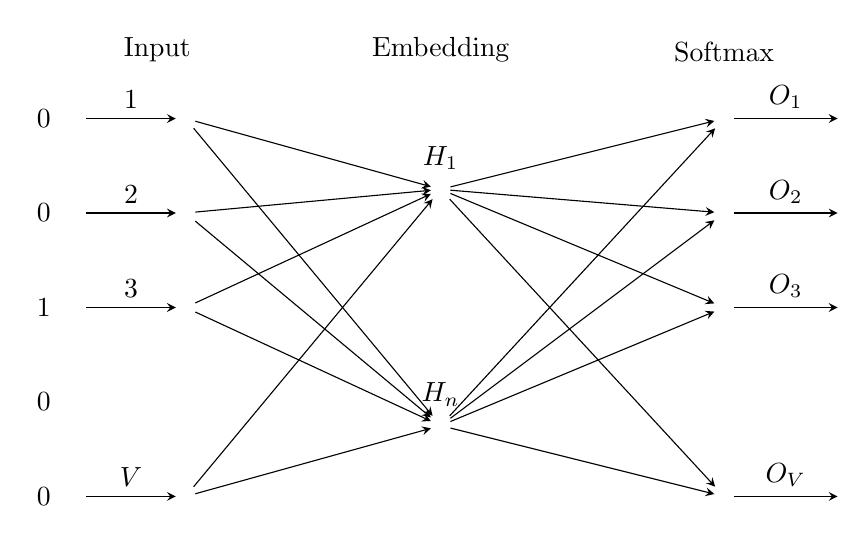
\begin{tikzpicture}[x=1.8cm, y=1.2cm, >=stealth]

\foreach \m/\l [count=\y] in {0, 0 , 1, 0 ,0}
  \node [every neinput/.try, neinput \m/.try] (input-\m) at (-0.8, 2.5-\y) {$\m$};
  
\foreach \m/\l [count=\y] in {1,2,3,missing,4}
  \node [every neuron/.try, neuron \m/.try] (input-\m) at (0.2,2.5-\y) {};

\foreach \m [count=\y] in {1,missing,2}
  \node [every neuron/.try, neuron \m/.try ] (hidden-\m) at (2,2-\y*1.25) {};

\foreach \m [count=\y] in {1,2, 3, missing,4}
  \node [every neuron/.try, neuron \m/.try ] (output-\m) at (4,2.5-\y) {};

\foreach \l [count=\i] in {1,2,3,V}
  \draw [<-] (input-\i) -- ++(-0.7,0)
    node [above, midway] {$\l$};

\foreach \l [count=\i] in {1, n}
  \node [above] at (hidden-\i.north) {$H_\l$};

\foreach \l [count=\i] in {1,2, 3, V}
  \draw [->] (output-\i) -- ++(0.8,0)
    node [above, midway] {$O_\l$};

\foreach \i in {1,...,4}
  \foreach \j in {1,...,2}
    \draw [->] (input-\i) -- (hidden-\j);

\foreach \i in {1,...,2}
  \foreach \j in {1,...,4}
    \draw [->] (hidden-\i) --(output-\j);

\foreach \l [count=\x from 0] in {Input, Embedding, Softmax}
  \node [align=center, above] at (\x*2,2) {\l };

\end{tikzpicture}

A vocabulary is fed into the neural network using one-hot encoding methods. For a vocabulary of size V, the input vector is of size 1xV

\end{frame}

\begin{frame}

\frametitle{ Neural Network Based Language Model: Architecture}

\begin{itemize}

\item The input variable is a one-hot encoding vector. If the vocabulary is of size V, an input vector is has V components $\mathnormal{\vec{x}=[0, 0, 0 ...1, ...0]}$ 
\item The hidden layer has $n$ neurons. The input weights matrix $\mathnormal{W}$ is of size $\mathnormal{V\times n}$
\item The output layer weights $\mathnormal{W}'$ matrix is of size $\mathnormal{n\times V}$
\item CBOW: take $2m$ words ( i.e. $\mathnormal{w_{c-m}}$, ...$\mathnormal{w_{c-1}}$, $\mathnormal{w_{c+1}}$, $\mathnormal{w_{c+m}}$) around the center word $\mathnormal{w_c}$ as input  $\mathnormal{w_c}$ is the target.
\item Skip-gram: take the center word $\mathnormal{w_c}$ as the input and the $2m$ words ( i.e. $\mathnormal{w_{c-m}}$, ...$\mathnormal{w_{c-1}}$, $\mathnormal{w_{c+1}}$, $\mathnormal{w_{c+m}}$) around it as the target.

\textbf{Reference}: \url {https://arxiv.org/pdf/1301.3781.pdf}

\end{itemize}

\end{frame}

\begin{frame}
\frametitle{Neural Network Based Language Model: Word Embedding}

The word representation/embedding can be calculated as 

$$\mathnormal{w_i=x_iW}$$

$\mathnormal{x_i}$ is the $\mathnormal{i^th}$ word in the dictionary, $\mathnormal{w_i}$ is the $\mathnormal{i^th}$ row in the input matrix $\mathnormal{W}$

\end{frame}

\end{document}
